In addition to the tools for working with mesh data described in previous chapters, $\tt{AMReX}$ also provides data structures and iterators for performing data-parallel particle simulations. Our approach is particularly suited to particles that interact with data defined on a (possibly adaptive) block-structured hierarchy of meshes. Example applications include Particle-in-Cell (PIC) simulations, Lagrangian tracers, or particles that exert drag forces onto a fluid, such as in multi-phase flow calculations. The overall goals of $\tt{AMReX}$'s particle tools are to allow users flexibility in specifying how the particle data is laid out in memory and to handle the parallel communication of particle data automatically. In the following sections, we give an overview of $\tt{AMReX}$'s particle classes and how to use them.

\section{The \tt{Particle}}
\label{sec:Particles:Particle}

The particle classes can be used by including the header $\tt{AMReX\_Particles.H}$. The most basic particle data structure is the particle itself: 

\begin{lstlisting}[language=cpp]
  Particle<3, 2> p;
\end{lstlisting}

This is a templated data type, designed to allow flexibility in the number and type of variables that the particles carry. The first template parameter is
the number of extra $\tt{Real}$ variables this particle will have (either single or double precision\footnote{Particles default to double-precision for their real data. To use single precision, compile your code with $\tt{USE\_SINGLE\_PRECISION\_PARTICLES=TRUE}$.}), while the second is the number of extra integer variables. 
It is important to note that this is the number of $\emph{extra}$ real and integer variables; a particle will always have at least $\tt{BL\_SPACEDIM}$ real components that store the particle's position and $\tt{2}$ integer components that store the particle's $\tt{id}$ and $\tt{cpu}$ numbers.\footnote{Note that $\tt{cpu}$ stores the number of the process the particle was $\emph{generated}$ on, not the one its currently assigned to. This number is set on initialization and never changes, just like the particle $\tt{id}$. In essence, the particles have two integer id numbers, and only the combination of the two is unique. This was done to facilitate the creation of particle initial conditions in parallel.}

The particle struct is designed to store these variables in a way that minimizes padding, which in practice means that the $\tt{Real}$ components always come first, and the integer components second. Additionally, the required particle variables are stored before the optional ones, for both the real and the integer components. For example, say we want to define a particle type that stores a mass, three velocity components, and two extra integer flags. Our particle struct would be set up like:

\begin{lstlisting}[language=cpp]
  Particle<4, 2> p;
\end{lstlisting}

and the order of the particle components in would be: x y z m vx vy vz id cpu flag1 flag2. \footnote{Note that for the extra particle components, which component refers to which
variable is an application-specific convention - the particles have 4 extra real comps, but which one is ``mass'' is up to the user. We suggest using an $\tt{enum}$ to keep these indices straight; please see amrex/Tutorials/Particles/ElectrostaticPIC/ElectrosticParticleContainer.H for an example of this.} 

\subsection{Setting Particle data}

The $\tt{Particle}$ struct provides a number of methods for getting and setting a particle's data. For the required particle components, there are special, named methods. For the 
``extra'' real and integer data, you can use the $\tt{rdata}$ and $\tt{idata}$ methods, respectively. 

\begin{lstlisting}[language=cpp]
  Particle<2, 2> p;

  p.pos(0) = 1.0;
  p.pos(1) = 2.0;
  p.pos(2) = 3.0;
  p.id() = 1;
  p.cpu()  = 0;

  // p.rdata(0) is the first extra real component, not the 
  // first real component overall
  p.rdata(0) = 5.0;
  p.rdata(1) = 5.0;

  // and likewise for p.idata(0);
  p.rdata(0) = 17;
  p.idata(1) = -64;  
\end{lstlisting}

\section{The \tt{ParticleContainer}}
\label{sec:Particles:ParticleContainer}
 
One particle by itself is not very useful. To do real calculations, a collection of particles needs to be defined, and the location of the particles within the AMR hierarchy
(and the corresponding MPI process) needs to be tracked as the particle positions change. To do this, we provide the $\tt{ParticleContainer}$ class:

\begin{lstlisting}[language=cpp]
  ParticleContainer<3, 2, 4, 4> mypc;
\end{lstlisting}
   
\subsection{Arrays-of-Structs and Structs-of-Arrays}

Like the $\tt{Particle}$ class itself, the $\tt{ParticleContainer}$ class is templated. The first two template parameters have the same meaning as before: they define the number of each type of variables that the particles in this container will store. Particles added to the container are stored in the Array-of-Structs (AoS) style. In addition, there are two more optional template parameters that allow the user to specify additional particle variables that will be stored in Struct-of-Array (SoA) form. The difference between Array-of-Struct and Struct-of-Array data is in how the data is laid out in memory. For the AoS data, all the variables associated with particle 1 are next to each other in memory, followed by all the variables associated with particle 2, and so on. For variables stored in SoA style, all the particle data for a given component is next to each other in memory, and each component is stored in a separate
array. For convenience, we (arbitrarily) refer to the components in the particle struct as particle $\emph{data}$, and components stored in the Struct-of-Arrays as particle
$\emph{attributes}$. See Figure~\ref{fig:particles:particle_arrays} for an illustration.

\begin{figure}
  \centering
  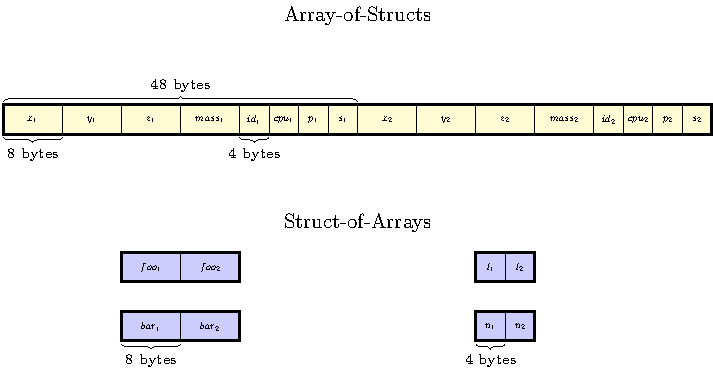
\includegraphics[width=\textwidth]{./Particle/particle_arrays.pdf}
  \caption{\label{fig:particles:particle_arrays} An illustration of how the particle data for a single tile is arranged in memory. This particle container has been defined with $\tt{NStructReal} = 1$, $\tt{NStructInt} = 2$, $\tt{NArrayReal} = 2$, and $\tt{NArrayInt} = 2$. In this case, each tile in the particle container has five arrays: one with the particle struct data, two additional real arrays, and two additional integer arrays. In the tile shown, there are only 2 particles. We have labelled the extra real data member of the particle struct to be ``mass'', while the extra integer members of the particle struct are labeled $p$, and $s$, for ``phase'' and ``state''. The variables in the real and integer arrays are labelled ``foo'', ``bar'', ``l'', and ``n'', respectively. We have assumed that the particles are double precision.}
\end{figure}

To see why the distinction between AoS and SoA data is important, consider the following extreme case. Say you have particles that carry 100 different components,
but that most of the time, you only need to do calculations involving 3 of them (say, the particle positions) at once. In this case, storing all 100 particle variables in the particle
struct is clearly inefficient, since most of the time you are reading 97 extra variables into cache that you will never use. By splitting up the particle variables into stuff that gets 
used all the time (stored in the AoS) and stuff that only gets used infrequently (stored in the SoA), you can in principle achieve much better cache reuse. Of course, the usage pattern of your application likely won't be so clear-cut. Flexibility in how the particle data is stored also makes it easier to interface between $\tt{AMReX}$ and already-existing Fortran subroutines.

Note that while ``extra'' particle data can be stored in either the SoA or AoS style, the particle positions and id numbers are $\emph{always}$ stored in the particle
structs. This is because these particle variables are special and used internally by $\tt{AMReX}$ to assign the particles to grids and to mark particles as valid or invalid, respectively.

\subsection{Constructing ParticleContainers}

A particle container is always associated with a particular set of AMR grids and a particular set of $\tt{DistributionMap}$s that describes which MPI processes those grids live on.
For example, if you only have one level, you can define a $\tt{ParticleContainer}$ to store particles on that level using the following constructor:

\begin{lstlisting}[language=cpp]
    ParticleContainer (const Geometry            & geom,
                       const DistributionMapping & dmap,
                       const BoxArray            & ba);
\end{lstlisting}

Or, if you have multiple levels, you can use following constructor instead:

\begin{lstlisting}[language=cpp]
    ParticleContainer (const Vector<Geometry>            & geom,
                       const Vector<DistributionMapping> & dmap,
                       const Vector<BoxArray>            & ba,
                       const Vector<int>                 & rr);
\end{lstlisting}

Note the set of grids used to define the $\tt{ParticleContainer}$ doesn't have to be the same set used to define the simulation's mesh data. However, it is often desirable to have
the two hierarchies track each other. If you are using an $\tt{AmrCore}$ class in your simulation (see Chapter~\ref{Chap:AmrCore}), you can achieve this by using 
the $\tt{AmrParticleContainer}$ class. The constructor for this class takes a pointer to your $\tt{AmrCore}$ derived class, instead:

\begin{lstlisting}[language=cpp]
  AmrTracerParticleContainer (AmrCore* amr_core);
\end{lstlisting}

In this case, the $\tt{Vector<BoxArray>}$ and $\tt{Vector<DistributionMap>}$ used by your $\tt{ParticleContainer}$ will be updated automatically to match those in
your $\tt{AmrCore}$. 

The $\tt{ParticleContainer}$ stores the particle data in a manner prescribed by the set of AMR grids used to define it. If tiling is turned off, then every grid has its own 
Array-of-Structs and Struct-of-Arrays. Which AMR grid a particle is assigned to is determined by examining its position and binning it, using the domain left edge as an offset. 
By default, a particle is assigned to the finest level that contains its position, although this behavior can be tweaked if desired. 
When tiling is enabled, then each $\emph{tile}$ gets its own Struct-of-Arrays and Array-of-Structs instead. Note that this is different than what happens with mesh data. With mesh data, the tiling is strictly logical; the data is laid out in memory the same whether tiling is turned on or off. With particle data, however, the particles are actually stored in different arrays when tiling is enabled. As with mesh data, the particle tile size can be tuned so that an entire tile's worth of particles will fit into a cache line at once.

Once the particles move, their data may no longer be in the right place in the container. They can be reassigned by calling the $\tt{Redistribute()}$ method of $\tt{ParticleContainer}$.
After calling this method, all the particles will be moved to their proper places in the container, and all invalid particles (particles with id set to $-1$) will be removed. All the 
MPI communication needed to do this happens automatically.

Application codes will likely want to create their own derived $\tt{ParticleContainer}$ class that specializes the template parameters and adds additional 
functionality, like setting the initial conditions, moving the particles, etc. See the amrex/Tutorials/Particles for examples of this.

\section{Initializing Particle Data}
\label{sec:Particles:Initializing}

In the following code snippet, we demonstrate how to set particle initial conditions for both SoA and AoS data. We loop over all the tiles using $\tt{MFIter}$, and add
as many particles as we want to each one.

\begin{lstlisting}[language=cpp]

for (MFIter mfi = MakeMFIter(lev); mfi.isValid(); ++mfi) {

    // ``particles'' starts off empty
    auto& particles = GetParticles(lev)[std::make_pair(mfi.index(),
                                        mfi.LocalTileIndex())];
 
    ParticleType p;
    p.id()   = ParticleType::NextID();
    p.cpu()  = ParallelDescriptor::MyProc();
    p.pos(0) = ...
    etc...

    // AoS real data
    p.rdata(0) = ...
    p.rdata(1)  = ...
         
    // AoS int data
    p.idata(0) = ...
    p.idata(1) = ...

    // Particle real attributes (SoA)
    std::array<double, 2> real_attribs;
    real_attribs[0] = ...
    real_attribs[1] = ...

    // Particle int attributes (SoA)
    std::array<int, 2> int_attribs;
    int_attribs[0] = ...
    int_attribs[1]  = ...
 
    particles.push_back(p);
    particles.push_back_real(real_attribs);
    particles.push_back_int(int_attribs);

    // ... add more particles if desired ...
  }

\end{lstlisting}

Often, it makes sense to have each process only generate particles that it owns, so that the particles are already in the right place in the container. 
In general, however, users may need to call $\tt{Redistribute()}$ after adding particles, if the processes generate particles they don't own (for example,
if the particle positions are perturbed from the cell centers and thus end up outside their parent grid).

\section{Iterating over Particles}
\label{sec:Particles:Iterating}

To iterate over the particles on a given level in your container, you can use the $\tt{ParIter}$ class, which comes in 
both const and non-const flavors. For example, to iterate over all the AoS data:

\begin{lstlisting}[language=cpp]

using MyParIter = ConstParIter<2*BL_SPACEDIM>;
for (MyParIter pti(pc, lev); pti.isValid(); ++pti) {
    const auto& particles = pti.GetArrayOfStructs();
    for (const auto& p : particles) {
        // do stuff with p...
    }
}
\end{lstlisting}

The outer loop will execute once every grid (or tile, if tiling is enabled) \emph{that contains particles}; grids or tiles
that don't have any particles will be skipped. You can also access the SoA data using the $\tt{ParIter}$ as follows:

\begin{lstlisting}[language=cpp]

using MyParIter = ParIter<0, 0, 2, 2>;
for (MyParIter pti(pc, lev); pti.isValid(); ++pti) {
    auto& particle_attributes = pti.GetStructOfArrays();
    Vector<Real>& real_comp0 = particle_attributes.GetRealData(0);
    Vector<int>&  int_comp1  = particle_attributes.GetIntData(1);
    for (int i = 0; i < pti.numParticles; ++i) {
        // do stuff with your SoA data...
    }
}
\end{lstlisting}

\section{Passing particle data into Fortran routines}
\label{sec:Particles:Fortran}

Because the $\tt{AMReX}$ particle struct is a Plain-Old-Data type, it is interoperable with $\tt{Fortran}$ when the $\tt{bind(C)}$
attribute is used. It is therefore possible to pass a grid or tile worth of particles into fortran routines for processing,
instead of iterating over them in C++. You can also define a Fortran derived type that is equivalent to C struct used for the
particles. For example:

\begin{lstlisting}[language=fortran]

    use amrex_fort_module, only: amrex_particle_real
    use iso_c_binding ,    only: c_int

    type, bind(C)  :: particle_t
       real(amrex_particle_real) :: pos(3)
       real(amrex_particle_real) :: vel(3)
       real(amrex_particle_real) :: acc(3)
       integer(c_int)   :: id
       integer(c_int)   :: cpu
    end type particle_t

\end{lstlisting}

is equivalent to particle struct you get with $\tt{Particle<6, 0>}$. Here, $\tt{amrex_particle_real}$ is either single or doubled precision, depending 
on whether $\tt{USE\_SINGLE\_PRECISION\_PARTICLES}$ is $\tt{TRUE}$ or not. We recommend always using this type in Fortran routines that work on particle
data to avoid hard-to-debug incompatibilities between floating point types.
See \S \ref{sec:Particles:Interacting}.
\section{Interacting with Mesh Data}
\label{sec:Particles:Interacting}

It is common to want to have the mesh communicate information to the particles and vice versa. For example, in Particle-in-Cell calculations, the particles deposit their charges onto the mesh, and later, the electric fields computed on the mesh are interpolated back to the particles. Below, we show examples of both these sorts of operations.

\begin{lstlisting}[language=cpp]

Ex.FillBoundary(gm.periodicity());
Ey.FillBoundary(gm.periodicity());
Ez.FillBoundary(gm.periodicity());
for (MyParIter pti(MyPC, lev); pti.isValid(); ++pti) {
    const Box& box = Ex[pti].validBox();

    const auto& particles = pti.GetArrayOfStructs();
    int nstride = particles.dataShape().first;
    const long np  = pti.numParticles();

    const FArrayBox& exfab = Ex[pti];
    const FArrayBox& eyfab = Ey[pti];
    const FArrayBox& ezfab = Ex[pti];

    interpolate_cic(particles.data(), nstride, np,
                    exfab.dataPtr(), eyfab.dataPtr(), ezfab.dataPtr(),
                    box.loVect(), box.hiVect(), plo, dx, &ng);
    }

\end{lstlisting}

Here, $\tt{interpolate\_cic}$ is a $\tt{Fortran}$ subroutine that actually performs the interpolation on a single box. $\tt{Ex}$, $\tt{Ey}$, and $\tt{Ez}$ are $\tt{MultiFab}$s
that contain the electric field data. These $\tt{MultiFab}$s must be defined with the correct number of ghost cells to perform the desired type of interpolation,
and we call $\tt{FillBoundary}$ prior to the Fortran call so that those ghost cells will be up-to-date. 

In this example, we have assumed that the $\tt{ParticleContainer}$ has been defined on the same grids as the electric field $\tt{MultiFabs}$, so that we use the $\tt{ParIter}$ to index into the $\tt{MultiFab}$s to get the data associated with current tile. If this is not the case, then an additional copy will need to be performed. However, if the particles are distributed in an extremely uneven fashion, it is possible that the load balancing improvements associated with the two-grid approach are worth the cost of the extra copy.

The inverse operation, in which the particles communicate data $\emph{to}$ the mesh, is quite similar:

\begin{lstlisting}[language=cpp]

rho.setVal(0.0, ng);
for (MyParIter pti(*this, lev); pti.isValid(); ++pti) {
    const Box& box = rho[pti].validbox();

    const auto& particles = pti.GetArrayOfStructs();
    int nstride = particles.dataShape().first;
    const long np  = pti.numParticles();

    FArrayBox& rhofab = (*rho[lev])[pti];

    deposit_cic(particles.data(), nstride, np, rhofab.dataPtr(), 
                box.loVect(), box.hiVect(), plo, dx);
    }

rho.SumBoundary(gm.periodicity());

\end{lstlisting}

As before, we loop over all our particles, calling a $\tt{Fortran}$ routine that deposits them on to the appropriate $\tt{FArrayBox}$. The FArrayBox's must have enough ghost cells to
cover the support of all the particles associated with them. Note that we call $\tt{SumBoundary}$ instead of $\tt{FillBoundary}$ after performing the deposition, to add up the charge 
in the ghost cells surrounding each Fab into the corresponding valid cells.

For a complete example of an electrostatic PIC calculation that includes static mesh refinement, please see amrex/Tutorials/Particles/ElectrostaticPIC.

\section{Short Range Forces}
\label{sec:Particles:ShortRange}

In a PIC calculation, the particles don't interact with each other directly; they only see each other through the mesh. An alternative use case is particles that exert short-range forces on each other. In this case, beyond some cut-off distance, the particles don't interact with each other and therefore don't need to be included in the force calculation. Our approach to these kind of particles is to fill ``neighbor buffers'' on each tile that contain copies of the particles on neighboring tiles that are within some number of cells $N_g$ of the tile boundaries. See Figure~\ref{fig:particles:neighbor_particles} for an illustration. By choosing the number of ghost cells to match the interaction radius of the particles, you can capture all of the neighbors that can possibly influence the particles in the valid region of the tile. The forces on the particles on different tiles can then be computed independently of each other using a variety of methods.

\begin{figure}
  \centering
  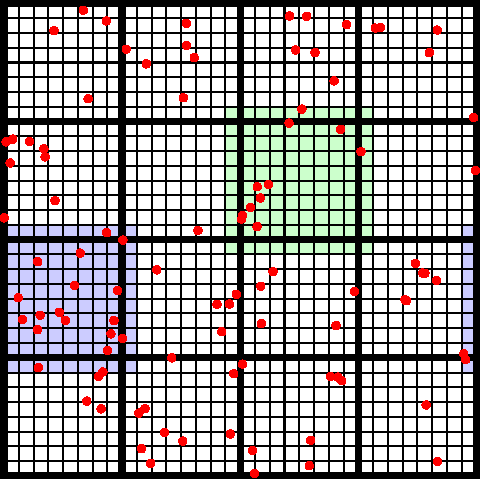
\includegraphics[width=0.75\textwidth]{./Particle/neighbor_particles.pdf}
  \caption{\label{fig:particles:neighbor_particles} An illustration of filling neighbor particles for short-range force calculations. Here, we have a domain consisting of one 32-by-32 grid, broken up into 8-by-8 tiles. The number of ghost cells is taken to be $1$. For the tile in green, particles on other tiles in the entire shaded region will copied and packed into the green tile's neighbor buffer. These particles can then be included in the force calculation. If the domain is periodic, particles in the grown region for the blue tile that lie on the other side of the domain will also be copied, and their positions will modified so that a naive distance calculation between valid particles and neighbors will be correct.
}
\end{figure}

For a $\tt{ParticleContainer}$ that does this neighbor finding, please see $\tt{NeighborParticleContainer}$ in amrex/Src/Particles/AMReX\_NeighborParticleContainer.H. This $\tt{ParticleContainer}$ has additional methods called $\tt{fillNeighbors()}$ and $\tt{clearNeighbors()}$ that fill the $\tt{neighbors}$ data structure with copies of the proper particles. A tutorial that uses these features is available at amrex/Tutorials/Particles/ShortRangeParticles. This tutorial computes the forces on a given tile via direct summation by passing the real and neighbor particles into a Fortran subroutine, as follows:

\begin{lstlisting}[language=cpp]

void ShortRangeParticleContainer::computeForces() {
    for (MyParIter pti(*this, lev); pti.isValid(); ++pti) {
        AoS& particles = pti.GetArrayOfStructs();
        int Np = particles.size();
        PairIndex index(pti.index(), pti.LocalTileIndex());
        int Nn = neighbors[index].size() / pdata_size;
        amrex_compute_forces(particles.data(), &Np,
                             neighbors[index].dataPtr(), &Nn);
    }
}

\end{lstlisting}

Alternatively, one can avoid doing a direct $N^2$ summation over the particles on a tile by binning the particles by cell and building a neighbor list. A tutorial that demonstrates this process is available at amrex/Tutorials/Particles/NeighborList. The data structure used to represent the neighbor lists is illustrated in Figure~\ref{fig:particles:neighbor_list}.

\begin{figure}
  \centering
  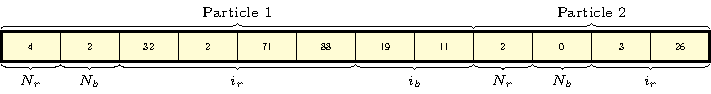
\includegraphics[width=\textwidth]{./Particle/neighbor_list.pdf}
  \caption{\label{fig:particles:neighbor_list} An illustration of the neighbor list data structure used by AMReX. The list for each tile is represented by an array of integers. The first number in the array is the number of real (i.e., not in the neighbor buffers) collision partners for the first particle on this tile, while the second is the number of collision partners from nearby tiles in the neighbor buffer. Based on the number of collision partners, the next several entries are the indices of the collision partners in the real and neighbor particle arrays, respectively. This pattern continues for all the particles on this tile.}
\end{figure}

This array can then be used to compute the forces on all the particles in one scan. Users can define their own $\tt{NeighborParticleContainer}$ subclasses that have their own collision criteria by overloading the virtual $\tt{check\_pair}$ function. For an example of this in action, please see the $\tt{NeighborList}$ Tutorial.

\section{Particle IO}
\label{sec:Particles:IO}

AMReX provides routines for writing particle data to disk for analysis, visualization, and for checkpoint / restart. The most important methods are the $\tt{WritePlotFile}$, $\tt{Checkpoint}$, and $\tt{Restart}$ methods of $\tt{ParticleContainer}$, which all use a parallel-aware binary file format for reading and writing particle data on a grid-by-grid basis. These methods are designed to complement the functions in $\tt{AMReX\_PlotFileUtil.H}$ for performing mesh data IO. For example:

\begin{lstlisting}[language=cpp]

    WriteMultiLevelPlotfile(``plt00000'', output_levs, GetVecOfConstPtrs(output),
                            varnames, geom, 0.0, level_steps, outputRR);
    pc.Checkpoint(``plt00000'', ``particle0'');

\end{lstlisting}

will create a plot file called ``plt00000'' and write the mesh data in $\tt{output}$ to it, and then write the particle data in a subdirectory called ``particle0''. There is also the $\tt{WriteAsciiFile}$ method, which writes the particles in a human-readable text format. This is mainly useful for testing and debugging.

The binary file format is currently readable by $\tt{yt}$. In additional, there is a Python conversion script in amrex/Tools/Py\_util/amrex\_particles\_to\_vtp that can convert both the ASCII and the binary particle files to a format readable by Paraview. See Chapter~\ref{Chap:Visualization} for more information on visualizing $\tt{AMReX}$ datasets, including those with particles. 
